\documentclass[conference,compsocconf]{IEEEtran}
\usepackage{amsmath,amssymb,amsfonts,float,graphicx,bm,psfrag,amsmath,amsthm}
\usepackage{algorithm, algorithmic,CJK,color,color,geometry,url}
\usepackage{graphicx,cite,bm,psfrag,amsmath}
\def\mmax{\mathop{\mbox{\scriptsize max}}}
\def\argmin{\mathop{\mbox{arg\,min}}}
\def\argmax{\mathop{\mbox{arg\,max}}}
\newcommand{\defequal}{\stackrel{\mathrm{def}}{=}}
\renewcommand{\vec}[1]{{\ensuremath{\boldsymbol{#1}}}}
\newcommand{\popt}{\ensuremath{P^{(K)}_{opt}}}
\renewcommand{\algorithmicrequire}{ \text{Input:}} %Use Input in the format of Algorithm
\renewcommand{\algorithmicensure}{ \text{Procedures:}} %UseOutput in the format of Algorithm
\newtheorem{mypro}{Proposition}
\IEEEoverridecommandlockouts
\pagestyle{plain}
\renewcommand{\algorithmicrequire}{ \textbf{Input:}} %Use Input in the format of Algorithm
\renewcommand{\algorithmicensure}{ \textbf{Procedures:}} %UseOutput in the format of Algorithm
\geometry{left=0.59in, right=0.59in, top=0.7in, bottom=0.69in}
\DeclareRobustCommand*{\IEEEauthorrefmark}[1]{%
	\raisebox{0pt}[0pt][0pt]{\textsuperscript{\footnotesize\ensuremath{#1}}}}
\def\BibTeX{{\rm B\kern-.05em{\sc i\kern-.025em b}\kern-.08em
		T\kern-.1667em\lower.7ex\hbox{E}\kern-.125emX}}
%\usepackage[colorlinks]{hyperref}
%\hypersetup{colorlinks=true,linkcolor=blue,filecolor=magenta,urlcolor=cyan}
\urlstyle{same}

%\usepackage{booktabs}
\usepackage[T1]{fontenc}
\usepackage[table]{ xcolor}
\setlength{\columnsep}{0.25in}
\begin{document}
	\title{Achieving the Highest Average User Data Rate in Wireless Network using Reinforcement Learning}
	\author{Qi Cao\IEEEauthorrefmark{1}, Mingqi Yuan\IEEEauthorrefmark{2}, Siliang Zeng\IEEEauthorrefmark{1}, Man-On Pun\IEEEauthorrefmark{1}\IEEEauthorrefmark{\dagger} and Yi Chen\IEEEauthorrefmark{1}\\
	\IEEEauthorrefmark{1}The Chinese University of Hong Kong, Shenzhen\\
	Guangdong, China, 518172\\
	\IEEEauthorrefmark{2}Mingqi's affilation
	\thanks{\IEEEauthorrefmark{\dagger}Corresponding author, email: SimonPun@cuhk.edu.cn. This work was supported, in part, by the Shenzhen Science and Technology Innovation Committee under Grant No. ZDSYS20170725140921348, ZDSYS201707251409055, the National Natural Science Foundation of China under Grant No. 61731018, 61701425 and Grant 2017ZT07X152.}}
\maketitle
	
	\begin{abstract}
		How to predict the wireless network-level performance such as the network capacity, the average user data rate, and the $5\%$-tile user data rate is a million-dollar question. In the literature, some pioneering works have been proposed by exploiting either the information theoretic techniques on the physical-layer (PHY) information or the Markov chain techniques on the multiple access control (MAC) layer information. However, since these mathematical model-driven approaches usually focus on a small part of the network structure, they cannot characterize the whole network performance. In this paper, we propose to utilize a data-driven machine learning approach to tackle this problem. More specifically, both PHY and MAC information is fed into a deep neural network (DNN) specifically designed for network-level performance prediction. Simulation results show that the network-level performance can be accurately predicted at the cost of higher computational complexity.
	\end{abstract}
	
	\begin{IEEEkeywords}
		Network-level performance prediction, Machine learning, Data-driven methodology
	\end{IEEEkeywords}
	
	\section{Introduction}
	
	Wireless communication network is a widely studied filed with rich expert knowledge. Within the system, various mathematical models have been built according to the different stages from the data generation to the final data reception, and each stage has drawn considerable attention from relevant researchers. However as a whole entity, the network-level  rather than link-level performance concerns the wireless operators most. By network-level performance, it could refer to the network capacity, average user data rate or 5\%-tile user data rate (the data rate of the worst 5\% users). That being said, how to predict the wireless network performance given all the available network status is still an significant problem looking to be unrevealed.
	
	It is worth mentioning that mathematical modeling is almost impossible to solve the problem. The technical challenges come from that: first, a wireless communication network is highly complex with many components and mechanisms, rendering the whole system analytically intractable; second, it is difficult to accurately describe channel transfer function, inter-cell interference and user distribution and movement etc; finally, network events are mostly stochastic such as user arrival, traffic load and channel variations. For these reasons, an option is to adopt over-simplified models to make them theoretically tractable, or alternatively to use a simulator, which is especially accepted in industry. Despite the fact that there are usually big discrepancies between simulations and filed tests, simulators is not a proper predictor that can be involved in real-time transmission decision making. It is because simulators still cannot get rid of the randomness, that is to say, starting from the same situation, simulators will give different outcomes. Also note that building a highly sophisticated simulator is very expensive and time-consuming, and using it is computationally demanding.
	
	On the other hand over the recent years, artificial intelligence (AI), specifically machine learning, has entered many industrial fields, be it traditional or emerging, and plays the role of a mighty competitor challenging existing rules and stereotypes. The great success in image and linguistic processing demonstrates the nearly cookie-cutter methodology is so efficient and formidable when dealing with big data. The exploding demand of data over the air loads increasingly more pressure on current mobile Internet, while model-driven solutions are leading us to the bottleneck. In such a context, the combination of machine learning and wireless communications is an essential and promising next step.The wireless communications system is a data-rich environment, where the data collection system has already been built naturally, gathering all kinds of well-defined overhead data by thousands of UEs and network entities. Despite that, very little improvement has been accomplished nowadays from the perspective of practical usage of the network data. 
	
	In this paper, we attempt to leverage DNNs to predict the network-level performance using both MAC and PHY layer information. The reason why we believe DNN is a better choice compared to model-driven methodology is that tractable models in wireless communication system are mostly assuming linear, stationary and with Gaussian statistics. While, the universal approximation theorem in deep learning suggests that with sufficient neurons, it is possible to approximate any continuous mapping \cite{marsland2014machine}. So with this ability, we expect a well trained DNN can absorb most  non-linearity and non-Gaussian factors in the system. Our main contributions are as follows:
	\begin{itemize}
		\item With a large number of various discrete/continuous counters and complicated operating mechanisms such as out loop link adaptation (OLLA) and proportional fairness (PF) user scheduling in wireless communication network, we demonstrate that using DNNs to predict network-level performance is possible. Specifically, we designed two DNN configurations respectively predicting the UE average throughput (UAT) and the ACK/NACK outcome of a transmission.
		\item Accurate labels are essential to train a DNN. Due to the stochastic nature beneath the system, the system can only provide labels with noises, that is, for the regression problem the label value can be far away from the actual value and for the classification problem the label can be totally wrong. Therefore, we develop a weighted co-teaching algorithm to tackle the noisy label problem. It shows using the algorithm, the training is more robust.
		\item Apart from that our trained DNN can reasonably predict the performance of the wireless communication network, we can also utilize it to provide new insights. Specifically, by altering the input counters, we are able to draw the MCS landscape, which can hardly be obtained before and provides us a new perspective to make decisions on transmission schemes.
	\end{itemize}
	

	
	In what follows, we introduce the task specifications and dataset establishment in Sec. II and the designed DNN configuration is detailed in Sec. III. The proposed training algorithm is elaborated in Sec. IV. Finally Sec. V presents the simulation results before conclusion is given in Sec. VI.
		
	\subsection{Related Works}
	There are early studies exploiting machine learning in radio resource management (RRM). For instance, power allocation in multi-user interference channels is a classic NP-hard problem in the field of wireless communications due to the combinatorial nature. With the goal being maximizing the weighted sum rate (WSR), the traditional convex optimization theory can reach solutions that are close to the global optimum using the iterative algorithm namely, weighted minimum mean-squared error (WMMSE). However, the WMMSE algorithm is of high complexity and thus time-consuming \cite{shi2011iteratively}. In \cite{sun2018learning}, a five-layer fully connected neural network is built to learn from the resulting solutions of WMMSE via supervised learning. On this basis, the work in \cite{liang2018towards} adopts the unsupervised learning method and uses the opposite of WSR as the loss function to train an ensembling deep neural networks (DNN), solving the same problem of power allocation. The results show that the sum rate obtained by the ensembling DNN in high SNR ($10$~dB) can even beat WMMSE. Even so, there is a big impediment hindering the practical implementation of such DNNs, which is the dynamic number of users. That is to say the above DNNs all have fixed input size to serve certain number of users. As the number users changes, especially when the number rises, the DNN is no longer valid. Nevertheless, it shows from a theoretical perspective that graph neural networks (GNN) can be a powerful solver to combinatorial problems, and GNN is totally scalable that they can adapt to dynamic number of entities \cite{sato2019approximation}. Thus, by using the a GNN to solve the same power allocation problem, the WSR is increased by more than 2 percent with respect to WMMSE which always finds a local optimum.
	
	The above power allocation methods require accurate channel state information (CSI). However, in the many current communication networks, the accurate CSI of the user equipment (UE) may not be available especially in the frequency division duplex system. A more common practice is that each UE feeds back its channel quality indicators (CQI) to the base station, and the base station determines the communication scheme based on the CQI. In \cite{ghadimi2017reinforcement}, an AI-based solution that uses only relatively accessible communication overhead data such as CQI to realize power allocation. Based on a two-cell model, the study applies reinforcement learning to allocate limited transmit power to $10$~UEs working in the same frequency band. The work shows that reinforcement learning is superior to the traditional algorithm in terms of the 5\%-tile and median UE data rates. Also, the work \cite{bruno2014robust} shows it is sufficient to effectively adjust the modulation and coding scheme (MCS) selection dynamically when the BS only needs the UE's CQI feedback.
	
	Apart from power allocation, a remarkable application of using deep learning in physical layer is the end-to-end learning wireless communication system. The basic idea behind is that a communication system is similar to a neural network, both of which have input and output side. Replacing the encoding/modulation and decoding/demodulation module with DNNs (named by autoencoder and autodecoder respectively), we are able to optimize the whole system as long as the back propagation can be enabled . It is interesting to observe that when the BS has redundant bits to interpret limited number of messages, the behavior of the trained autoencoder is like doing channel coding. However when the BS lacks sufficient number of bits to describe the messages, the autoencoder is more like doing modulation \cite{o2017introduction,o2017deep}. To enable the back propagation, the channel model must represent all non-linearity in the real system and it must do so in a differentiable way. However in real-world system, it is difficult to obtain such an accurate analytic representation. To overcome the missing channel gradient problem, \cite{o2018physical} proposes to use another DNN to mimic the the signal transfer. Since with both input and output signals, it is feasible to  train the channel approximation DNN via supervised learning. 
	
	Note that matching learning also gets involved in many other aspects of RRM.  For instance, in \cite{wei2018joint} the actor-critic reinforcement learning algorithm is used to handle user scheduling and content caching at the same time. Besides in a mobile edge computing network, study \cite{huang2019deep} uses a deep reinforcement learning algorithm to handle the tasks offloading problem which is of NP-hardness.
	
	However to the best of our knowledge, current studies have not addressed the following two essential questions:
	\begin{itemize}
		\item How much insight can be derived from communication big data to benefit the whole system?
		\item Is machine learning still competent in the context of more complex and practical multi-layer wireless network structures?
	\end{itemize}
	
\section{System Model}
\subsection{Simulator Basics}\label{setup}

\begin{figure}
	\centering
	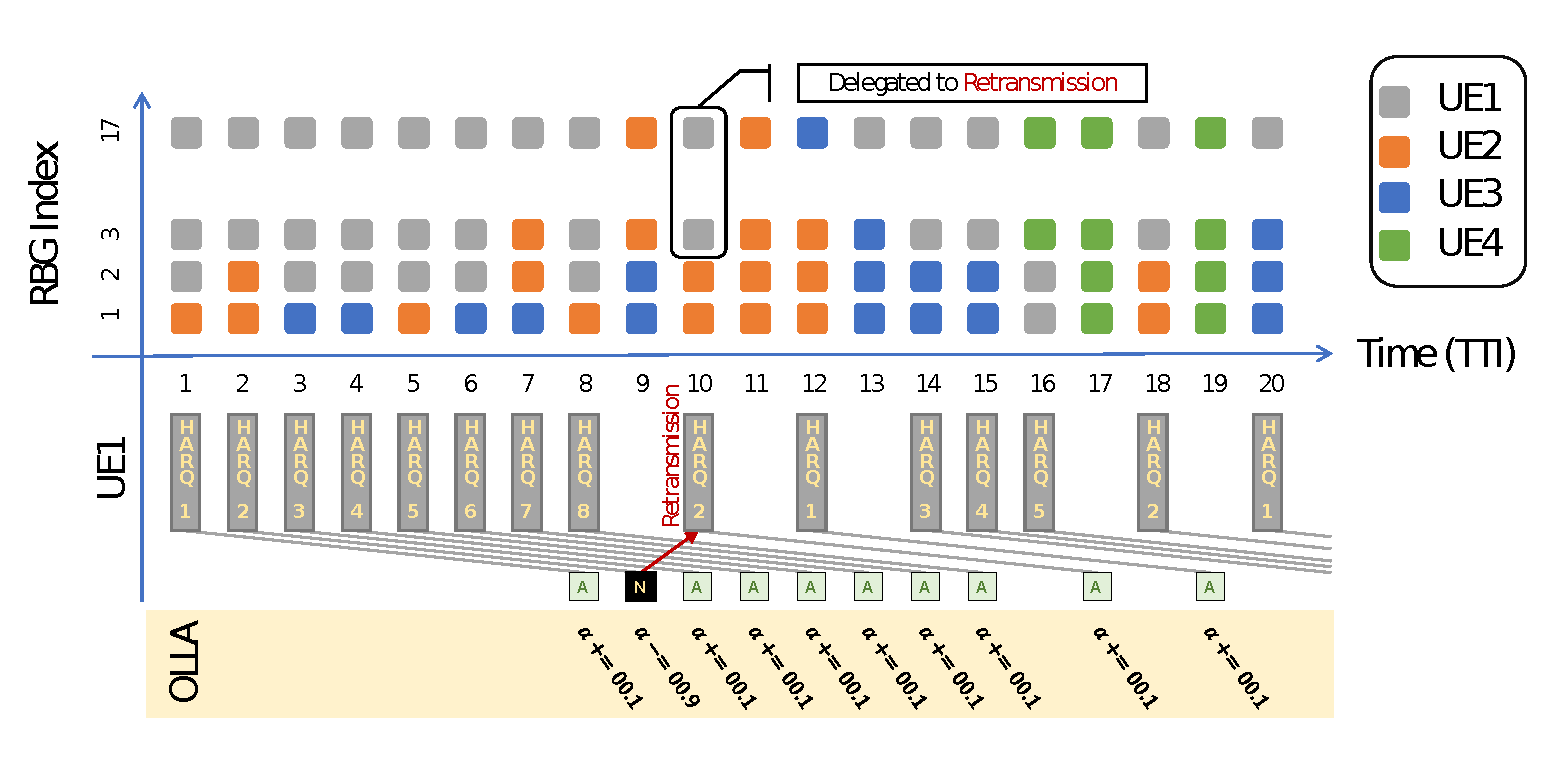
\includegraphics[width=1\linewidth]{Figs/system.eps}
	\caption{Network Mechanisms}
	\label{sys}
\end{figure}

We begin with the introduce of some basic information about the communication systems that we are dealing with. Specifically, we simulate a $20$-second single-cell wireless communications process, where the system is working at the LTE FDD mode at $2$~GHz frequency band. $50$ resource blocks (RB) allocated into $17$ resource block groups (RBG) utilizing $10$~MHz bandwidth are set up to serve downlink UEs with arrival rate equal to five UEs per second. The base station is equipped with two transmit/receive antennas respectively while UEs are equipped with one transmit antenna and two receive antennas. Being under bursty buffer traffic, the system randomly initializes the buffer size between $0.5$~Kbytes and $3$~Mbytes for each arrived UE. In addition, the noise power density is at $-174$~dBm/Hz, and the transmit power of each RB is fixed at $18$~dBm. In what follows, 

\subsubsection{Out Loop Link Adaptation}
The LTE protocol allows	the UE to suggest an appropriate MCS to be used in the next transmission, which is aimed at targeting a certain the block error rate (BLER). To propose such a suggestion, the UE actually selects its wanted MCS by sending back a CQI value as a quantized reference. Typically, each CQI representing a signal-to-noise ratio (SNR) interval is periodically measured and reported. Thus MCSs are indeed selected by mapping the received instantaneous SNR into its interval.The tricky part about MCS selection is that it cannot be either too aggressive (high) or too conservative (low). The higher level the MCS is adopted, the larger TB size is supported, but also the higher BLER is, and vice versa. Empirically, the MCS achieving a BLER of 90\% is mostly accepted, as the expected size of the TB that can be successfully transmitted is the largest at this point. 

However, this mapping rule is not sufficient to sensitively compensate the discrepancy between the chosen MCS and the optimal MCS for different UEs. Note that every UE may have its specificity, for instance, aged devices might require relatively lower MCS to the same channel condition compared to new devices. Thus to make the compensation, the BS allows the OLLA algorithm to carry out to offset a CQI value $q$, which is
\begin{equation}
\bar{q}=\left[q+\alpha\right],
\end{equation}
being $[\cdot]$, the rounding operation and $\bar{q}$ the offset CQI readily for MCS selection. Note that $\alpha$ is the adjustment coefficient which is dynamically updated every time an ACK/NACK message is fed back. Specifically, let $\mathfrak{K}$ denote the ACK/NACK flag, being 1 for ACK and 0 for NACK. To achieve the BLER of 90\%, the update rule is given by 

\begin{equation}
\alpha=
\begin{cases}
\alpha+0.01, & \mathfrak{K} = 1, \\
\alpha-0.09, & \mathfrak{K} = 0.
\end{cases}
\end{equation}
Note that UEs' CQI level is an RB-wise measurement, and each CQI is one-to-one mapped to an MCS associating with unique spectral efficiency (SE), see Appendix \ref{A1} for details. Thus we directly assume $\mathcal{M}(\bar{q})$ denotes the mapping from the offset CQI $\bar{q}$ to its SE, then, the estimated data rate of UE $n$ in RBG $k$ can be obtained by
\begin{equation}
R_{n,k}=\sum_{\ell\in \mathcal{G}(k)} B\mathcal{M}(\bar{q}_{n,\ell}),
\end{equation}
where $\mathcal{G}(k)$ is the set of all RBs in RBG $k$, and $\ell$ is the index of an RB, and $\bar{q}_{n,\ell}$ is the offset CQI level of UE $n$ in RB $\ell$. The BS adopts a default MCS when the CQI is not given, which especially happens at the beginning of a transmission. 


\subsubsection{Hybrid Automatic Repeat reQuest and Retransmission}
When the TB for a UE is readily to be transmitted, a HARQ process will be triggered, which means the data will be shifted from the buffer to the HARQ buffer and they will stay there until being successfully transmitted or dropped. The  BS prepares eight HARQ processes for each UE, and when a new transmission task comes, it always chooses the HARQ process with the smallest possible index. Seven TTIs after the data have been radiated out, the BS will receive an ACK/NACK message from the corresponding UE. In the case of ACK, the TB being successfully transmitted and thus cleared on the BS, the HARQ process terminates. In the case of NACK, a retransmission is activated. The original RBGs will be delegated to conduct the retransmission and thus temporally unavailable for PF user scheduling. The MCS chosen for the retransmission must be the same as preceding to ensure that the source data can be reloaded to the delegated RBGs gain. Five times of consecutively failed retransmission on the same HARQ process forces it to terminate and drop the TB, and that literally causes the so-called packet loss in common sense.

For instance in Fig.\ref{sys}, UE1 started a transmission using HARQ	process 2 in TTI 2. After seven TTIs, the BS received a NACK message, meaning the transmission was failed and thus initiated a retransmission in TTI 10 using the same HARQ process and RBGs.
It is worth mentioning that if the situation of SNR allows, the BS can send two TBs to one UE at the same TTI using two codewords.

\subsection{Problem Formulation}

\section{Proposed Reinforcement Learning Solution}

\subsection{Environment and Agent}

\subsection{RBGnet Configuration}

\subsection{Training Method}


\section{Numerical Results}

\subsection{Beach Mark Schemes}
\subsubsection{Opportunistic User Scheduling}
\subsubsection{Propotional Fairness User Scheduling}
To balance the system throughput and fairness, a user scheduling called proportional fairness is proposed in [], where the scheduling is achieved by allocate RBGs to different UEs. Any UE with a non-empty buffer on the BS side is a candidate to each RBG, and each RBG independently sort all UEs according to their PF values. Denote the PF value of UE $n$ on RBG $k$ within transmission time interval (TTI) $i$ by $\beta_{n,k}[i]$ computed as
\begin{equation}
\beta_{n,k}[i]=\frac{R_{n,k}[i]}{\bar{T}_n[i]},
\label{eq1}
\end{equation}
where $\bar{T}_n[i]$ is the UE's moving average historical throughput which can be expressed as
\begin{equation}
\bar{T_n}[i]=\left(1-\gamma\right)\bar{T}_n[i-1]+\gamma T_n[i-1].
\label{eq:2}
\end{equation}
In Eq. (\ref{eq:2}), $\gamma$ is the moving average coefficient, which is usually very small, and $T_n[i-1]$ is the actual TB size of UE $n$ in TTI $i-1$ interpreted as how many number of bits is sent in last TTI. We sometimes omit the TTI index for brevity in the sequel. The UEs with higher PF value are with higher priorities to capture the RBG, and the PF value of a UE to different RBGs can be different.  To avoid allocate more RBGs to a UE than it needs, each RBG $k$ finds its highest PF value among all UEs $\mathop{\max}_{n}\left\{\beta_{n,k}\right\}$, and the RBG allocation is done one by one according to the ordered set in descending fashion
$\left\{\mathop{\max}_{n}\left\{\beta_{n,k}\right\}\right\}$. Each time when an RBG is allocated to a UE, say $n^*$, the system checks if $n^*$ obtained enough RBG to convey all its buffer data. If so, $n^*$ will be removed from remaining RBGs' lists, which always happens when the buffer of UE $n^*$ is about to be emptied.

When multiple RBGs are allocated to the a UE, they are utilized to convey one data packet (Transport Block, TB) with the same MCS. That is to say, even though the estimated data rate $R_{n,k}$ is adopted in the user scheduling, but the size of the TB loading on the RBG might differ. Suppose $\{\bar{q}_{n,\ell}\}$ with size $L$ is the set of all RBs allocated to UE $n$, then the actual TB size is written as
\begin{equation}
T_n=LB\mathcal{M}\left(\bigg\lfloor\frac{1}{L}\sum_{\ell}\bar{q}_{n,\ell}\bigg\rfloor\right),
\end{equation}
where $\lfloor\cdot\rfloor$ is the floor function. However if a UE fails to acquire any RB, $T_n$ will be equal to zero at the current TTI, as a consequence, the moving average throughput will goes down and the priority of the UE in all RBG will increase.

\section{Conclusion}
    
\bibliographystyle{ieeetr}
\bibliography{reference}
\end{document}


